\documentclass{article}
\usepackage[utf8]{vietnam}
% Gói chèn ảnh
\usepackage{graphicx}
% Ký hiệu toán
\usepackage{amsmath}
% Ký tự đặc biệt
\usepackage{amssymb}
% Định nghĩa, định lý
\usepackage{amsthm}

\begin{document}
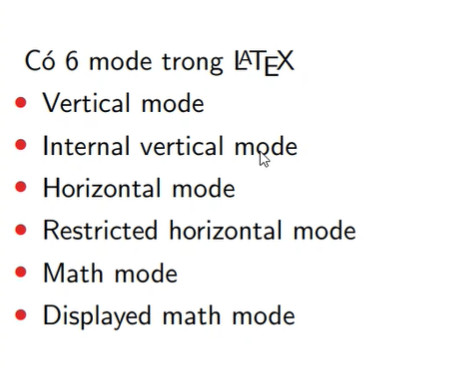
\includegraphics[scale=0.6]{image/latex-mode.jpg}\\
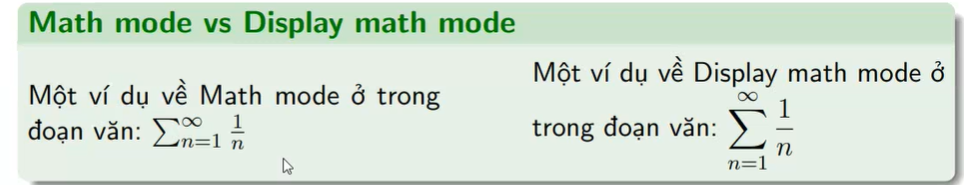
\includegraphics[scale=0.3]{image/math-mode.jpg}\\
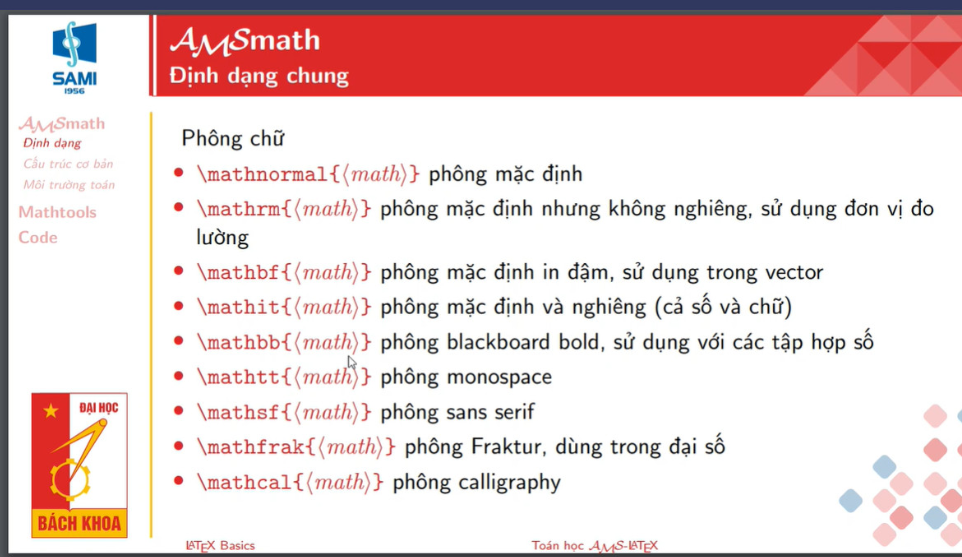
\includegraphics[scale=0.6]{image/dinh-dang-chung.png}\\
Văn bản toán học đầu tiên : 
\begin{itemize}
	\item $\mathnormal{123 f(x)}$
	\item $\mathrm{123 f(x)}$
	\item $\mathbf{123 f(x)}$
	\item $\mathit{123 f(x)}$
	\item $\mathbb{R Z C Q}$
	\item $\mathtt{R Z C Q}$
	\item $\mathfrak{R Z C Q}$
	\item $\mathcal{R Z C Q}$
\end{itemize}

% Kiểu chữ
% \displaystyle: kiểu chữ trong dạng display
$$\frac{x^2+y^2}{z^2}$$
% \textstyle: kiểu chữ trong dạng text
$$\textstyle\frac{x^2+y^2}{z^2}$$
% \scriptstyle: kiểu chữ trong dạng text
$$\scriptstyle\frac{x^2+y^2}{z^2}$$
% \scriptscriptstyle: kiểu chữ trong dạng text
$$\scriptscriptstyle\frac{x^2+y^2}{z^2}$$

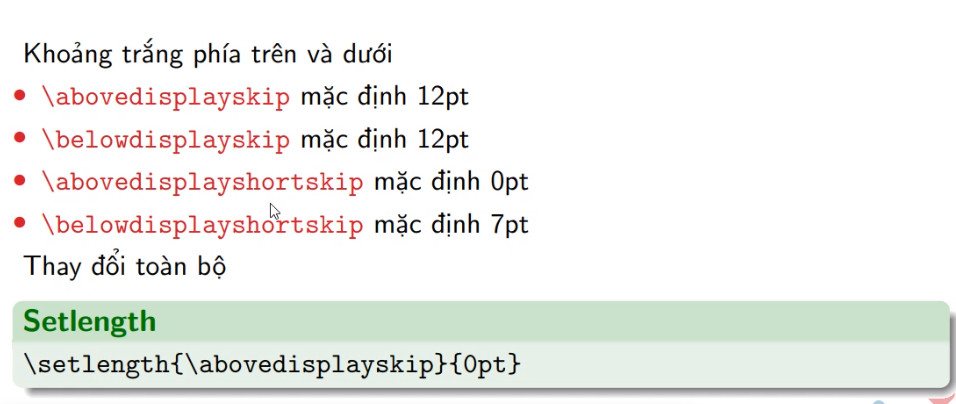
\includegraphics[scale=0.3]{image/khoang-trang.jpg}

Biểu diễn công thức toán học
\abovedisplayskip=20pt
$$\displaystyle \frac{x^2+y^2}{z^2}$$

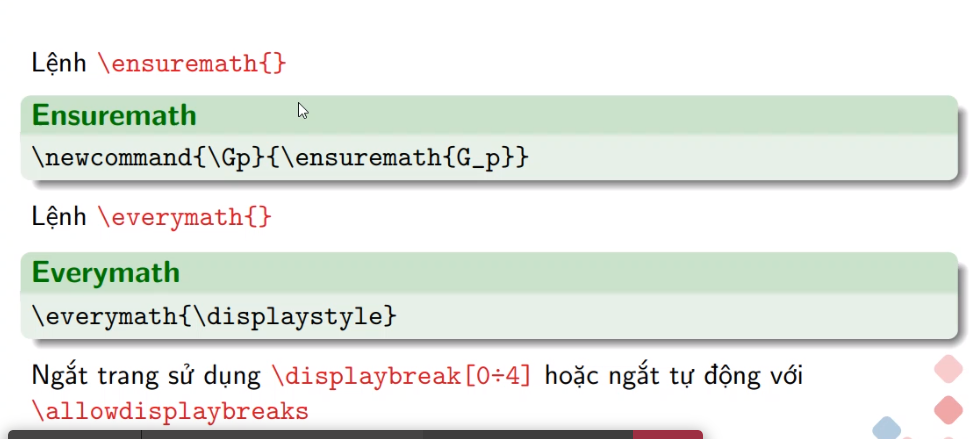
\includegraphics[scale=0.6]{image/ensuremth.png}

\newpage

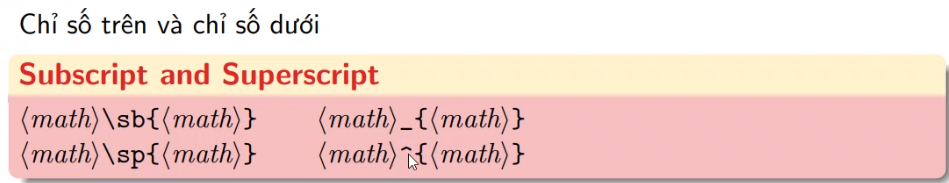
\includegraphics[scale=0.6]{image/subscript.png}

\vspace{1cm}

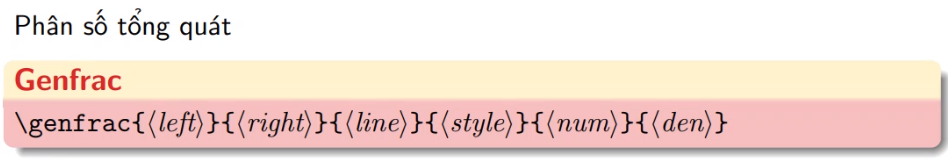
\includegraphics[scale=0.6]{image/genfrac.png}
$$\genfrac{(}{)}{0pt}{}{123}{456}$$

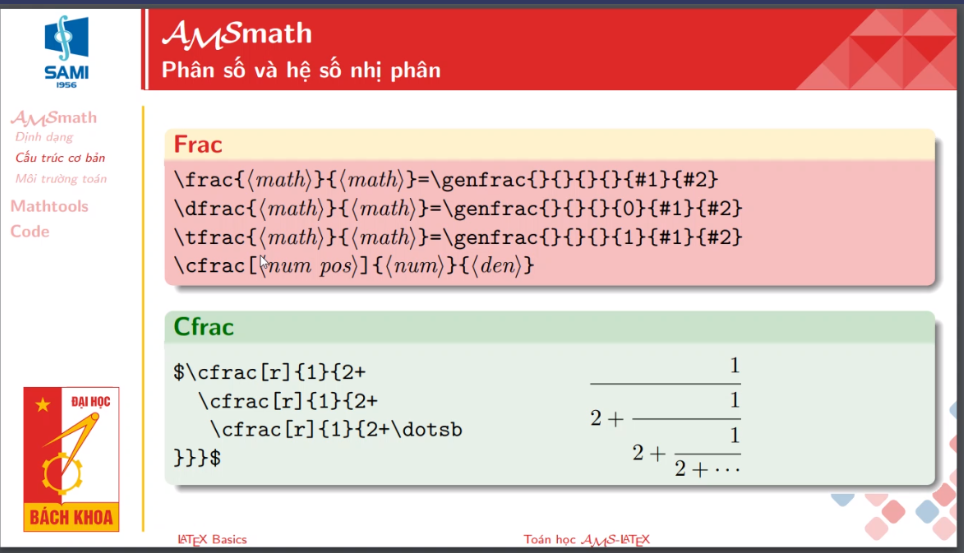
\includegraphics[scale=0.6]{image/frac.png}

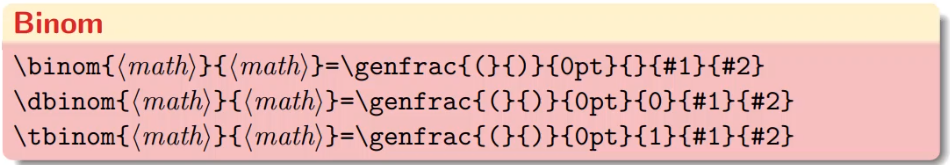
\includegraphics[scale=0.6]{image/binom.png}

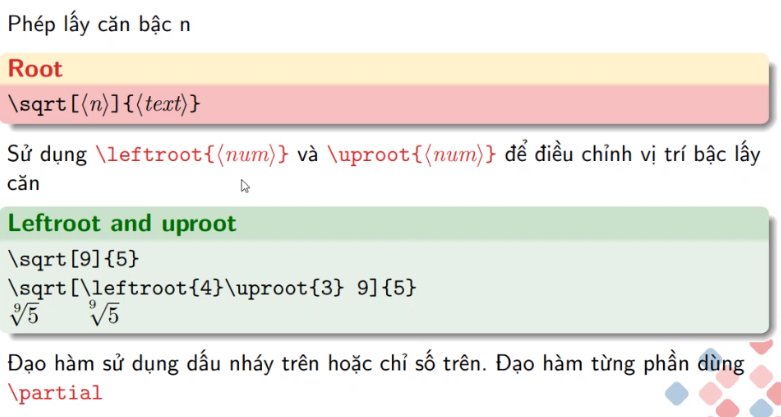
\includegraphics[scale=0.6]{image/root.png}

Biểu diễn căn thức, đạo hàm:
$$ \sqrt[\frac{1}{2}]{12345}$$ 
$$ \sqrt[\uproot{4} \frac{1}{2}]{12345}$$ 

Đạo hàm riêng : $\partial$

Tích phân trong latex:
$$ \int_{12}^{30} x^2+2x+3$$
Thêm các loại tích phân đặc biệt :
$$ \oint $$
$$\iint$$ 
$$\iiint \idotsint $$
Cách sử dụng limits:
$$ \int_a^b x^3+x+1 $$
$$ \int\limits_a^b x^3+x+1 $$
$$ \sum_{x=1}^\infty \frac{1}{n}$$
$$ \sum\nolimits_{x=1}^\infty \frac{1}{n}$$

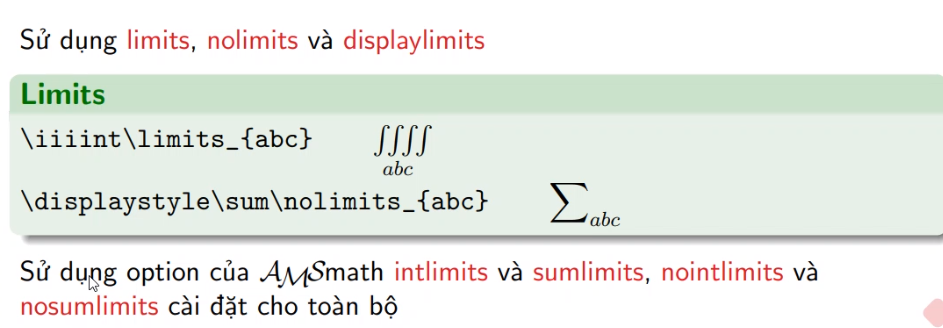
\includegraphics[scale=0.6]{image/limit.png}

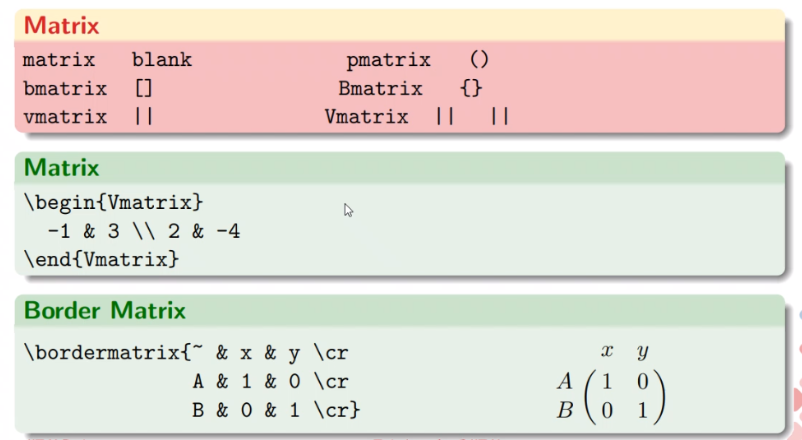
\includegraphics[scale=0.6]{image/matrix.png}

Môi trường matrix :
% Định thức ma trận
$\begin{vmatrix}
	-1 & 3\\2 & -4
\end{vmatrix}$

% Chuẩn ma trận
$\begin{Vmatrix}
	-1 & 3\\
	2 & -4
\end{Vmatrix}$\\

Bao ma trận :
$
\bordermatrix{~ & x & y \cr
A & 1 & 0 \cr
B & 0 & 1 \cr}
$

Dấu ngoặc ở trong môi trường toán:

$$\left( \frac{x^2}{y^2} \right) 
$$

Các loại dấu chấm :
$$\dots \quad  \ldots \quad  \cdots \quad  \vdots \quad  \ddots$$

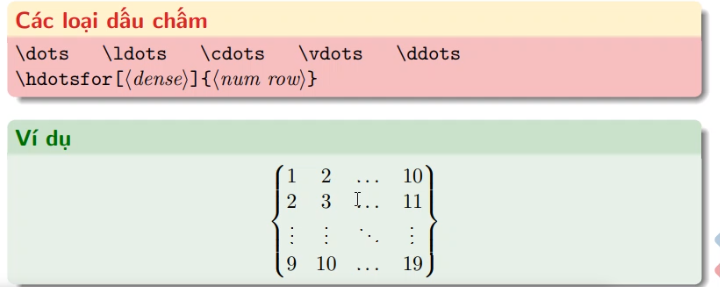
\includegraphics[scale=0.6]{image/dot.png}

Biểu diễn ma trận  với hdotsfor:
$$
\begin{matrix}
	1&3&3\\
	\hdotsfor[]{3}\\
	4&6&7
\end{matrix}
$$

Môi trường array:
$\begin{array}{c|c}
	1 & 2 \\ \hline
	3 & 4
\end{array}$

Môi trường cases:
$\begin{cases}
	\exp{x} & \text{if } x \geq 0 \\
	1 & \text{if } x < 0
\end{cases}$

\end{document}